% !TEX root = ../disertace.tex
%!TEX encoding = UTF-8 Unicode

\chapter{Conclusion}
\label{sec:conclusion}
\todo

\section{z LRE}

We have annotated multi-word lexemes and named entities on a part of PDT 2.0. We use tectogrammatical tree structures of MWEs for automatic pre-annotation. In Section~\ref{sec:annot:pre} we show that the richer the tectogrammatical annotation the better the possibilities for automatic pre-annotation that minimizes human errors. In the analysis of inter-annotator agreement we show that a weighted measure that accounts for partial agreement as well as estimation of maximal agreement is needed. 

The resulting $\kappa_w^U = 0.644$ is statistically significant and should gradually improve as we clean up the annotation lexicon, more entries are pre-annotated automatically, and further types of pre-annotation are employed.

The metodology of MWE annotation we developed enables precise pre-annotation by automatically extracted tectogramatical tree structures. We have shown that this pre-annotation does improve annotation speed and should improve also agreement. Initially only manual annotation will become more automatic and our pre-annotation procedures will mark more occurances. This leaves the annotator only to decide weather this meaning is correct or not.

---------

\section{rozpracovat}
\xx{Co jsme udelali:} hypoteza o tekto stromech MWE, anotacni nastroj, datovy format pro data, vyuziti hypotezy v predanotaci, \semlex, jeho datova representace, t-stromecky v semlexu, extension -- zobrazeni anotaci a vyhledavani v nich; prvni data, o kterych vime, kde muze i uzivatel hledat shodu a neshodu, apod. (umozneno skvelymi nastroji jinych: PML, tred, pml-tq). Hypoteza potvrzena? Mimochodem anotaci nalezeny chyby v PDT, nektere systematickeho razeni (chybejici uzly v koordinacich?), a take se ukazalo, ze nas blokovaly nedokoncenosti t-lemmat (deminutiva, prechylovani).

\xx{Zhodnotit vysledky toho, ze nekdy se vyplati anotovat rucne}, a nekdy ne: pripad jmen osob. Zjevne jsme udelali chybu, ze jsme to neanalyzovali takto (viz data od PaSi - EB) drive a nepredanotovali zbytek automaticky podle PDT. Ovsem, nasli by pak anotatori to, co nasli, kdyz by si zvykli na velmi vysokou uspesnost predanotace?

\xx{Pravdepodobnostni pristup k idiomaticnosti} -- mira, nikoliv kategorialni velicina s hodnotami nic, frazem, idiom, ..., ale zaroven mame miru pro mereni vazene shody. 

\section{Further analysis of annotation logs}
\label{sec:conc:logs}
Considering the price of annotations, it is interesting, how much the annotation process itself stays out of focus of the researchers who create annotated data. Reading the papers and listening to presentations on NLP conferences and the various annotation workshops, one cannot help but see this approach: The data is very interesting, so let us just create it somehow. Almost never is there any published information on the annotation process, factors that influence quality of data, or the price of the results. 

Logs are a  very good source of this valuable information. They can provide an insight into what is actually going on during annotation. Thorough statistical analysis of the logs can provide unbiased information that is hard to get any other way. Better analysis of logs together with s-files can perhaps improve estimation of the real cost of annotations. We have done this during annotations to some extent \see{sec:time-analysis}, but our method is not particularly sophisticated and we just more or less guessed the fluency constant for the annotation intervals.
 
As a small sample of what can be done with the data, we present some further information on the time aspect of annotation work. We decided to have a look at the distribution of times between two consecutive annotation actions. We hoped that it can give us more information for properly handling the fluency of annotation intervals discussed in \Sref{sec:time-analysis}. 

We leave it to real statisticians to examine the data more carefully. What is however quite striking in the plots in \Fref{fig:hist} and \Fref{fig:hist-detail}, is the similarity of the histograms. Even though they are not normalised to disregard the different amount of data annotated by each person, the distributions point to a remarkable similarity in behaviour of all three annotators. Compare for instance the distribution for the times up to five seconds. We do not have any explanation or even hypotheses for the uniform raise at 1 second\footnote{histograms actually indicate a lower bound of an interval. 2 seconds thus means $\langle1, 2)$, etc.}, drop at 2, raise at three, etc. It seems to be an interesting point to examine, however.

\begin{figure}[htbp]
   \centering
   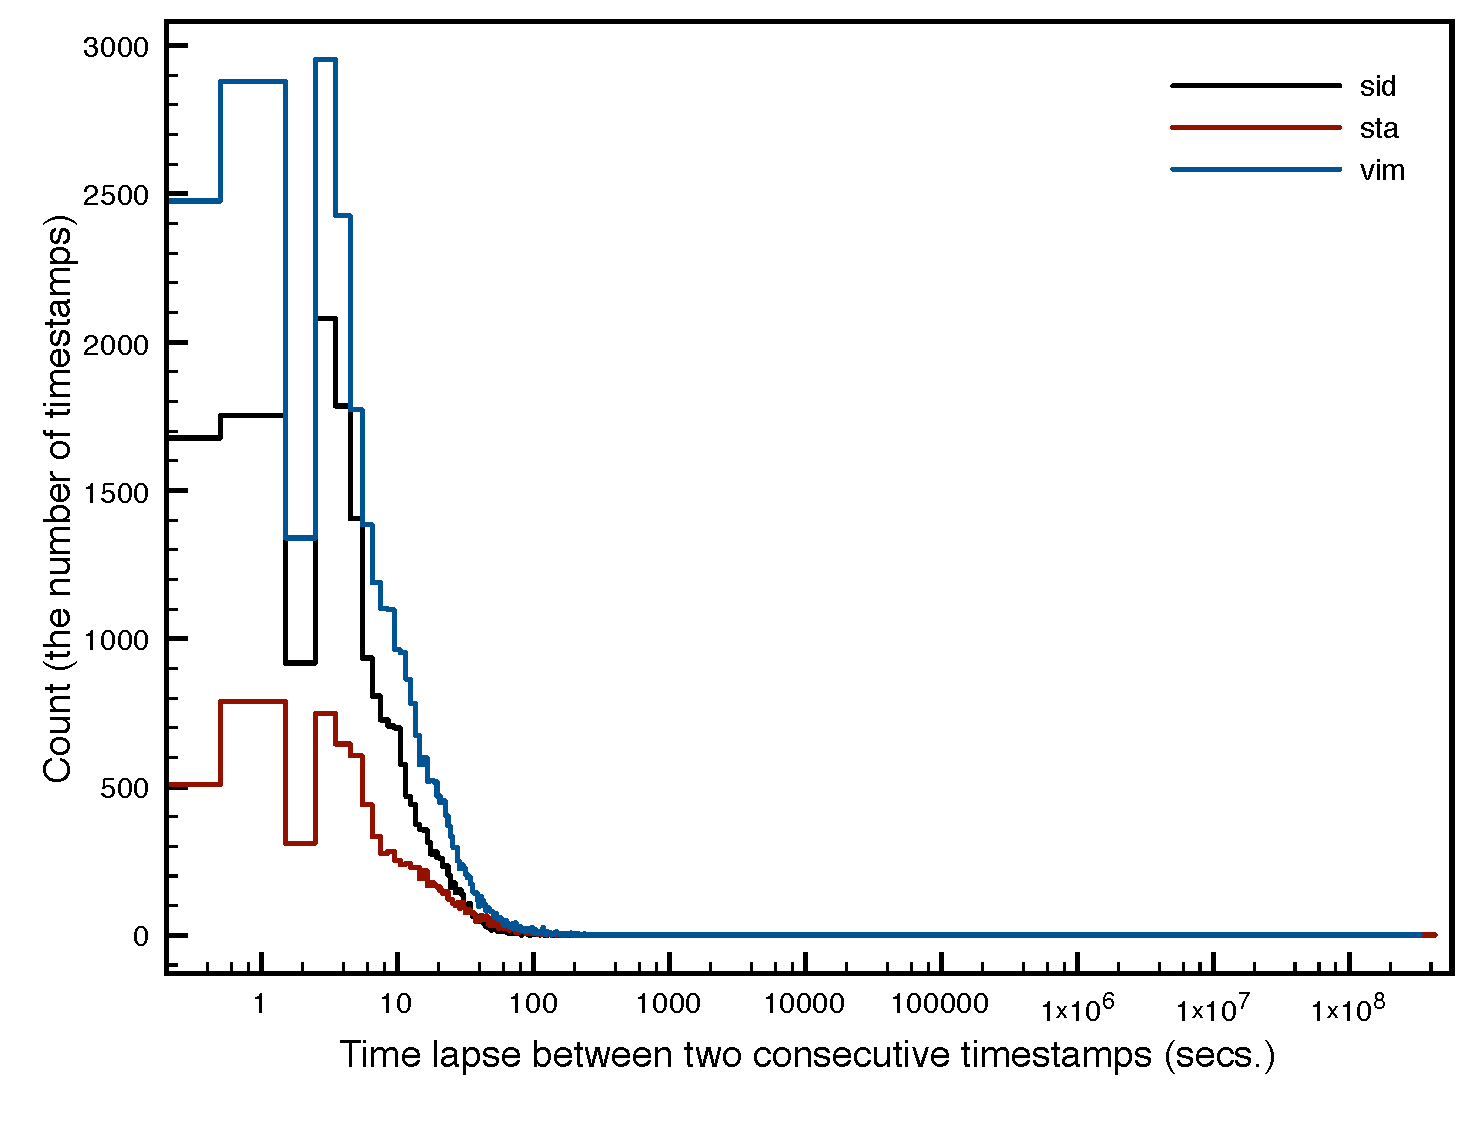
\includegraphics[width=.8\textwidth]{images/speed/histograms} 
   \caption{A histogram showing how many times ($y$) did an annotator place the next tag exactly $x$ seconds after the previous one.} 
   \label{fig:hist}
\end{figure}

\begin{figure}[htbp]
   \centering
   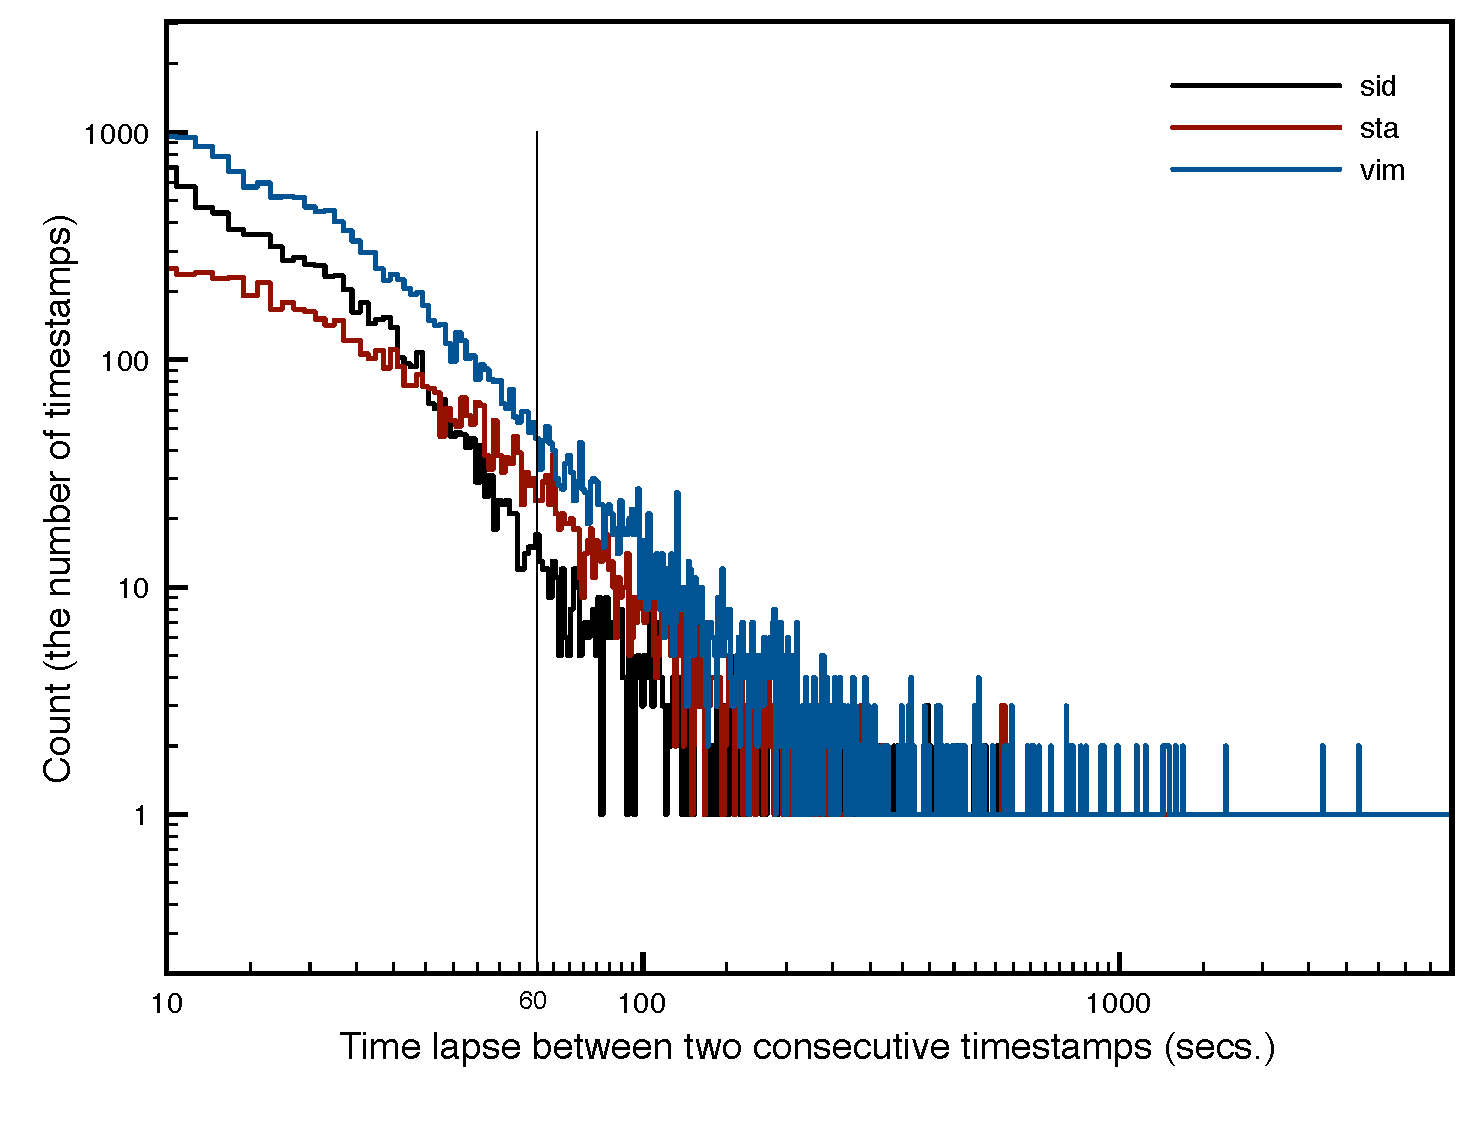
\includegraphics[width=.8\textwidth]{images/speed/histograms-detail} 
   \caption{Detail of the histogram in \Fref{fig:hist} in an interval where we have placed our \emph{fluency} value for the preliminary experiment with clustering of work into annotation intervals ($f=60$, see \Sref{sec:time-analysis} and \Fref{fig:speed}).}
\label{fig:hist-detail}
\end{figure}


But the analysis can go further and, to formulate the problem in economic terms, try to examine in general what factors influence the price of a (correct) tag. What is the relation of speed, length of work intervals, time of day, order of processing of the file, and other factors? We give only a very brief glimpse of one of the factors -- speed of annotations, but in our opinion thorough statistical analysis of log files is an important source of information also for future annotation projects. It may be possible to maximise the efficiency of annotations by experimentally identifying the positive and negative factors. Some of the factors can be quite universal, such as worse concentration after $n$ hours of work, but some may be quite individual (e.g. working in the morning, or on Saturdays\ldots). If some positive and negative factors influencing annotation can indeed be identified, annotation guidelines, both for the project and for the individual annotator can be appropriately modified to maximise the positive and avoid the negative factors.

It is of course possible, that no such factors can actually be estimated reliably, at last from our data. But currently we are in position to seriously examine the possibility and to find out, which is more than has been done until now. From the little that we can see now, there is already some interesting data that requires interpretation.
